\documentclass{article}
\usepackage[T1]{fontenc}
\usepackage[utf8]{inputenc}
\usepackage{ismir}
\usepackage{amsmath,cite,url}
\usepackage{graphicx}
\usepackage{booktabs}
\newcommand{\NTempo}{290}
\newcommand{\AccOneAC}{39.3}
\newcommand{\AccTwoAC}{87.2}
\newcommand{\AccOnePulse}{19.0}
\newcommand{\AccTwoPulse}{76.2}
\newcommand{\AccOnePrior}{66.6}
\newcommand{\AccTwoPrior}{89.7}
\newcommand{\AccOneIOI}{47.6}
\newcommand{\AccTwoIOI}{85.9}
\newcommand{\AccOneLibrosa}{70.7}
\newcommand{\AccTwoLibrosa}{87.2}
\newcommand{\AccOneMadmom}{81.4}
\newcommand{\AccTwoMadmom}{96.9}
\newcommand{\HalfAC}{34.5}
\newcommand{\MadmomMs}{2.1}
\newcommand{\LibrosaMs}{46}
\newcommand{\AccOneStretchMin}{67.2}
\newcommand{\AccOneStretchMax}{74.1}
\newcommand{\RelErrFour}{1.7}
\newcommand{\RelErrTwelve}{1.1}
\newcommand{\SpliceMAE}{18.7}
\newcommand{\SettleMed}{0.3}
\newcommand{\SettleFrac}{62}
\newcommand{\NChange}{58}
\newcommand{\DetFoldMed}{1.2}
\newcommand{\DetFoldTwo}{75}
\newcommand{\DetRawMed}{2.2}
\newcommand{\DetRawTwo}{46}
\newcommand{\BestTight}{300}
\newcommand{\DPF}{0.76}
\newcommand{\DPCML}{0.57}
\newcommand{\DPAML}{0.85}
\newcommand{\DPOracleF}{0.84}
\newcommand{\DPOracleCML}{0.85}
\newcommand{\DPOracleAML}{0.89}
\newcommand{\LibF}{0.76}
\newcommand{\LibCML}{0.62}
\newcommand{\LibAML}{0.81}
\newcommand{\MadF}{0.88}
\newcommand{\MadCML}{0.79}
\newcommand{\MadAML}{0.94}
\newcommand{\NNF}{0.64}
\newcommand{\NNCML}{0.23}
\newcommand{\NNAML}{0.47}
\newcommand{\NNDBNF}{0.83}
\newcommand{\NNDBNCML}{0.71}
\newcommand{\NNDBNAML}{0.88}
\newcommand{\NBeat}{290}
\newcommand{\AgreeMed}{0.98}
\newcommand{\AgreeShare}{74}
\newcommand{\AgreeRawMed}{0.96}
\newcommand{\LibBeatTime}{0.23}
\newcommand{\MadTime}{6.4}
\newcommand{\NNDBNTime}{0.51}
\newcommand{\MLPTime}{0.39}
\newcommand{\DPTime}{0.35}
\newcommand{\DegClean}{0.79}
\newcommand{\DegOrClean}{0.89}
\newcommand{\PercClean}{0.80}
\newcommand{\MadDegClean}{0.90}
\newcommand{\DegNoiseZero}{0.80}
\newcommand{\DegOrNoiseZero}{0.91}
\newcommand{\PercNoiseZero}{0.78}
\newcommand{\MadDegNoiseZero}{0.90}
\newcommand{\DegNoiseMinusTen}{0.60}
\newcommand{\DegOrNoiseMinusTen}{0.75}
\newcommand{\PercNoiseMinusTen}{0.53}
\newcommand{\MadDegNoiseMinusTen}{0.68}
\newcommand{\DegWhite}{0.79}
\newcommand{\DegOrWhite}{0.90}
\newcommand{\PercWhite}{0.78}
\newcommand{\MadDegWhite}{0.88}
\newcommand{\DegLPOne}{0.75}
\newcommand{\DegOrLPOne}{0.86}
\newcommand{\PercLPOne}{0.73}
\newcommand{\MadDegLPOne}{0.85}
\newcommand{\DegLPFour}{0.78}
\newcommand{\DegOrLPFour}{0.88}
\newcommand{\PercLPFour}{0.78}
\newcommand{\MadDegLPFour}{0.90}
\newcommand{\DegMPThree}{0.79}
\newcommand{\DegOrMPThree}{0.88}
\newcommand{\PercMPThree}{0.80}
\newcommand{\MadDegMPThree}{0.90}
\newcommand{\NDeg}{58}
\newcommand{\DBOracle}{0.34}
\newcommand{\NDown}{290}
\newcommand{\DBFirst}{0.26}
\newcommand{\DBNN}{0.17}
\newcommand{\DBNNFirst}{0.17}
\newcommand{\DBMadJoint}{0.65}
\newcommand{\DBMadBar}{0.76}

%% method paragraphs, one macro per member, reused by all three reports
\newcommand{\MethodIrai}{%
\textbf{Autocorrelation tempo estimation (Irai).} The autocorrelation
\begin{equation}
r(\tau) = \sum_n o(n)\,o(n+\tau)
\end{equation}
is computed with the FFT, and the plain estimate is $\hat{T} = 60 f_r/\tau^\ast$ for the lag $\tau^\ast$ with the largest $r(\tau)$ between 40 and 250\,BPM. A pulse train stage following \cite{percival} scores the ten strongest autocorrelation peaks by the best phase-aligned match of pulses at $\tau$, $1.5\tau$ and $2\tau$. The octave decision stage weights each of the ten candidates $\hat{T}_k$ by a log-normal prior,
\begin{equation}
s_k = r(\tau_k)\, \exp\!\Big(-\tfrac{1}{2}\log_2^2 \frac{\hat{T}_k}{120}\Big),
\label{eq:prior}
\end{equation}
and returns the candidate with the largest $s_k$. An inter-onset-interval (IOI) histogram of picked onsets is a simple baseline. For Objective 2, clips are time-stretched with the ffmpeg \texttt{atempo} filter, which keeps the pitch, so the true tempo becomes $fT$ for a factor $f$. The local estimator applies the octave decision to sliding windows of length $W$ with a hop of 1\,s. Spliced clips join a part stretched by $f_1$ to a part stretched by $f_2$ with a 10\,ms crossfade, at 15\,s of the source for the tracking test and at a random point between 10 and 20\,s for the detection test, in both directions. The change detector folds the local tempo curve into one octave around its median, $u_i = \mathrm{wrap}(\log_2(\hat{T}_i/\mathrm{med}\,\hat{T}))$ with $\mathrm{wrap}$ to $[-\tfrac12, \tfrac12)$, so that octave jumps do not look like changes, and picks the split point that minimises the squared deviation of $u$ from the median of each side.}

\newcommand{\MethodNalluraj}{%
\textbf{Dynamic programming beat tracking (Nalluraj).} Following Ellis \cite{ellis}, the tempo is estimated from the autocorrelation of $o(n)$ weighted by a log-Gaussian window around 120\,BPM, giving a beat period $p$ in frames. The best score of a beat sequence ending at frame $t$ is
\begin{equation}
C(t) = o(t) + \max_{\tau \in [t-2p,\, t-p/2]} \Big( C(\tau) - \alpha \log^2\!\frac{t-\tau}{p} \Big),
\label{eq:dp}
\end{equation}
where the tightness $\alpha$ sets how strongly the tracker keeps an even spacing. The beat sequence is recovered by backtracking from the best frame near the end. The tracker is run with the estimated tempo and with the oracle tempo from the annotations, which separates tempo errors from beat placement errors. For Objective 2, clips are degraded with pink noise at 20 to $-10$\,dB SNR, white noise at 0\,dB, a sixth-order zero-phase Butterworth low pass filter at 4, 2 and 1\,kHz, and MP3 encoding at 128, 64 and 32\,kbps with ffmpeg. The percussive envelope applies the same spectral flux to the percussive part of a median-filter harmonic-percussive separation (17-frame kernels).}

\newcommand{\MethodUsha}{%
\textbf{Neural network beat tracking (Usha).} Each frame is described by its 40 log-mel values and their positive differences, normalised per clip and stacked over $\pm 4$ frames (720 features). A multilayer perceptron (MLP) with two hidden layers of 128 and 64 units predicts the probability $a(n)$ that frame $n$ lies within one frame of a beat. Negative frames are subsampled to three times the positive frames, and training stops early on a 10\% validation part. Beats are the peaks of the smoothed activation that exceed a local mean by 0.05 and are at least 0.2\,s apart. As a second decoder, $a(n)$ is passed to madmom's DBN beat tracker \cite{madmom, downbeat}, which only uses our activation and no madmom network.

\textbf{Downbeat finder (Usha).} Given beats $b_1, \dots, b_K$ and a bar length $L$ from the annotations, the finder takes the peak of the low-frequency onset envelope $o_{\mathrm{low}}$ (six lowest mel bands, below about 200\,Hz) within 50\,ms of each beat and chooses the bar phase
\begin{equation}
\phi^\ast = \arg\max_{\phi \in \{0,\dots,L-1\}} \frac{1}{|\{k : k \equiv \phi\}|}\sum_{k \equiv \phi \,(\mathrm{mod}\, L)} o_{\mathrm{low}}(b_k),
\label{eq:down}
\end{equation}
on the idea that the kick drum and bass mark the downbeat. A baseline takes the first beat as the downbeat.}

\newcommand{\PITable}{%
\begin{table}[t]
\centering\small\setlength{\tabcolsep}{5pt}
\begin{tabular}{@{}llccccc@{}}
\toprule
Member & Obj. & PI1 & PI2 & PI3 & PI4 & PI5 \\
\midrule
Irai & 1 & D & P & D$^\ast$ & D & D \\
Irai & 2 & D & D & D & D & D \\
Nalluraj & 1 & D & D & D & D & -- \\
Nalluraj & 2 & D & D & P & D & -- \\
Usha & 1 & D & P & D & P & -- \\
Usha & 2 & D & D & D & D & -- \\
\bottomrule
\end{tabular}
\caption{Status of all performance indicators. D: done, P: partly done, --: not started. PI1 and PI2 are basic, PI3 and PI4 expected, PI5 advanced. $^\ast$Done, with a negative result.}
\label{tab:pi}
\end{table}}

\newcommand{\TimelineTable}{%
\begin{table}[t]
\centering\small\setlength{\tabcolsep}{3pt}
\begin{tabular}{@{}lp{0.80\columnwidth}@{}}
\toprule
Week & Plan (status) \\
\midrule
1--2 & Spec, repository, data, shared front end, basic methods (done) \\
3--4 & Evaluation on GTZAN, librosa and madmom comparisons (done) \\
5 & TCN in PyTorch (Usha); 1D State Space tracker under the same tests (Nalluraj, Usha); GiantSteps tempo (Irai) \\
6 & Advanced goals: tempo following and automatic tightness (Nalluraj), TCN with downbeat output and stretch augmentation (Usha), pulse train fix and change detection on real tempo changes (Irai) \\
7 & Final report and presentation (Dec 1--7) \\
\bottomrule
\end{tabular}
\caption{Revised timeline. Weeks 5 and 6 are Nov 17--23 and Nov 24--30.}
\label{tab:time}
\end{table}}

\newcommand{\MeIntro}{This report is Irai's individual submission: Section~\ref{sec:me} is his status report, and Section~\ref{sec:team} summarises the rest of the group.}

\title{Tempo Estimation under Tempo Changes: Progress Report}

\threeauthors
  {Irai Kumaran Sivanesan}{University of Victoria}
  {Nalluraj Babu}{University of Victoria}
  {Usha Sundaresan Manivannan}{University of Victoria}

\sloppy
\begin{document}
\maketitle

\begin{abstract}
This is the progress report of Irai Kumaran Sivanesan for the CSC 475/575 group project DP2\_B on tempo estimation and beat tracking. My part is an autocorrelation tempo estimator built from scratch and a study of tempo estimation when the tempo changes. On the artist-filtered GTZAN test split (\NTempo{} clips) the plain estimator reaches Accuracy1 \AccOneAC{}\%, mostly losing to octave errors. A pulse train stage made this worse, while a simple octave decision raised Accuracy1 to \AccOnePrior{}\%, close to librosa (\AccOneLibrosa{}\%) but below madmom (\AccOneMadmom{}\%). Accuracy is stable on clips stretched by 0.8 to 1.2, and a sliding-window estimator with an octave-folded change detector locates a sudden tempo change within 2\,s in \DetFoldTwo{}\% of spliced clips. I also report the status of my teammates and our revised plan.
\end{abstract}

\section{Introduction}

Tempo estimation finds how fast a piece of music is, in beats per minute (BPM), and beat tracking finds the times at which a listener would tap along. Both are basic tasks in music information retrieval and a first step for downbeat tracking, chord recognition and structure analysis \cite{tutorial}. Our group (Default Project 2, DP2\_B) set three goals in the design specification: build one complete method per member from scratch, compare these methods with existing tools, and study three known weak spots: changing tempo, degraded audio and the bar level (downbeats).

Each member owns one method and one study. Irai Kumaran Sivanesan works on tempo estimation and tempo changes, Nalluraj Babu on dynamic programming beat tracking and degraded audio, and Usha Sundaresan Manivannan on neural network beat tracking and downbeats. \MeIntro{} All code, result files and the scripts that make every number, table and figure in this report are in our repository.\footnote{\url{https://github.com/Iraikumaran/beat-tracking}, branch \texttt{Dev}.}

\section{Related Work}

Most tempo and beat systems first compute an onset detection function \cite{bello} and then look for periodicities in it. Gouyon et al. \cite{gouyon} compared tempo induction algorithms, introduced the Accuracy1 and Accuracy2 measures, and showed that choosing half or double the correct tempo is the most common error. Percival and Tzanetakis \cite{percival} proposed a streamlined estimator based on autocorrelation followed by cross-correlation with pulse trains. Ellis \cite{ellis} framed beat tracking as dynamic programming over an onset envelope, the method behind the beat tracker of librosa \cite{librosa}. For music with changing tempo, Grosche and M\"uller \cite{plp} estimate a local pulse in short windows.

Neural networks now give the best results. B\"ock et al. \cite{downbeat} predict beat and downbeat activations with recurrent networks and decode them with a dynamic Bayesian network (DBN), as implemented in madmom \cite{madmom}. Krebs et al. \cite{krebsbar} find downbeats from beat-synchronous features. Davies and B\"ock \cite{tcn} showed that temporal convolutional networks (TCNs) are accurate and small, and Heydari et al. \cite{heydari} reduced decoding cost with a one dimensional state space. Davies et al. \cite{tutorial} give a practical overview of all of these methods. Mauch and Ewert \cite{degradation} showed that MIR systems, beat trackers included, lose accuracy under common audio degradations.

Evaluation follows Davies et al. \cite{daviseval} with the reference implementation in mir\_eval \cite{mireval}. GTZAN was introduced by Tzanetakis and Cook \cite{gtzan}; Sturm \cite{sturm} documents its faults, and Kereliuk et al. \cite{kereliuk} proposed the artist-filtered split we use. The beat and downbeat annotations come from Marchand et al. \cite{marchand}. GiantSteps Tempo \cite{giantsteps} is the second dataset in our plan.

\section{Data and Evaluation}

We use the GTZAN audio with the beat, downbeat and tempo annotations of the gtzan\_tempo\_beat repository \cite{tutorial, marchand}. All results are on the artist-filtered test split of Kereliuk et al. \cite{kereliuk} (\NTempo{} clips of 30\,s, all ten genres). The neural network is trained on 160 clips from the matching training and validation splits (16 per genre), so no test artist is seen in training. The studies on tempo changes and degraded audio use an evenly spaced subset of \NDeg{} test clips (every fifth clip, all genres). The reference tempo of a clip is $T = 60/\mathrm{median}(\Delta b)$, where $\Delta b$ are the annotated inter-beat intervals.

For a tempo estimate $\hat{T}$, Accuracy1 counts $|\hat{T}-T| \le 0.04\,T$, and Accuracy2 also accepts $\hat{T}$ within 4\% of $kT$ for $k \in \{2, 3, \tfrac{1}{2}, \tfrac{1}{3}\}$. For beats and downbeats we report the F-measure with a $\pm 70$\,ms tolerance window,
\begin{equation}
F = \frac{2PR}{P+R},
\end{equation}
where $P$ and $R$ are the precision and recall of the estimated beats, together with the continuity measures CMLt and AMLt \cite{daviseval}. CMLt asks for a continuous sequence at the correct metrical level, and AMLt also accepts double, half and off-beat sequences. Beats in the first 5\,s are ignored; for downbeats they are kept.

\textbf{Shared front end.} Audio is resampled to 22.05\,kHz and a short-time Fourier transform is computed with a 2048-sample Hann window and a hop of 256 samples ($f_r = 86.1$ frames per second). The magnitude is mapped to 40 mel bands and compressed as $M(f,n) = \log(1 + 100\,X_{\mathrm{mel}}(f,n))$. The onset envelope is the half-wave rectified spectral flux
\begin{equation}
o(n) = \sum_f \max\big(0, M(f,n) - M(f,n-1)\big),
\end{equation}
with a moving average removed and the result normalised. Our own methods use only NumPy, SciPy and scikit-learn; librosa \cite{librosa} and madmom \cite{madmom} are used only as reference systems.

\textbf{Repeatability.} Every experiment was run twice from a clean results folder on the same machine. Apart from run times, the two runs gave identical result files, and they also matched the files that each member had produced on their own laptop (two of 6090 rows in the tightness sweep differ, both at $\alpha = 3000$, by floating point effects).


\section{Methods}

\MethodIrai

\begin{table}[t]
\centering\small\setlength{\tabcolsep}{3.5pt}
\begin{tabular}{@{}lccccc@{}}
\toprule
Method & Acc1 & Acc2 & Half & Dbl. & ms \\
\midrule
\csname @@input\endcsname ../figures/tab_tempo.tex
\bottomrule
\end{tabular}
\caption{Tempo estimation on the GTZAN test split (\%, \NTempo{} clips). Half and Dbl.\ give the share of clips estimated at half or double the reference tempo; ms is the mean run time per clip on one laptop, for our methods without the shared onset envelope.}
\label{tab:tempo}
\end{table}

\begin{figure}[t]
\centering
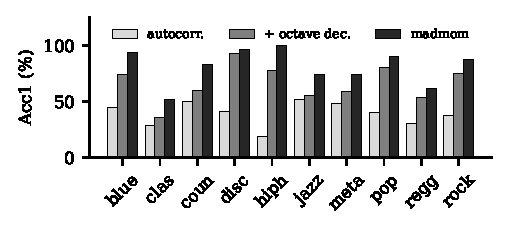
\includegraphics[width=\columnwidth]{../figures/fig_tempo_genre.pdf}
\caption{Accuracy1 per genre for the plain estimator, the estimator with octave decision, and madmom.}
\label{fig:tgenre}
\end{figure}

\section{Individual Status Report: Irai Kumaran Sivanesan}
\label{sec:me}

\textbf{Objective 1: autocorrelation tempo estimator.}
\emph{PI1 (basic, done).} The estimator runs on all \NTempo{} test clips in about a millisecond per clip once the onset envelope is computed.
\emph{PI2 (basic, partly done).} Accuracy1, Accuracy2 and an octave error label are reported on GTZAN (Table~\ref{tab:tempo}). The plain estimator reaches Acc1 \AccOneAC{}\% but Acc2 \AccTwoAC{}\%, so most of its errors are octave errors; \HalfAC{}\% of the clips are estimated at half the tempo. GiantSteps is still missing because its audio is downloaded from an online store's preview server with the dataset script, which was blocked in our first setup.
\emph{PI3 (expected, done with a negative result).} The pulse train stage lowered Acc1 to \AccOnePulse{}\%. Our scoring favours slow periods, because a pulse train at $2\tau$ also lines up with every second beat. Three variants (phase contrast, subdivision energy and normalised pulse trains) did not beat the plain estimator.
\emph{PI4 (expected, done).} On the same clips and machine, the IOI baseline reaches \AccOneIOI{}\%, librosa \AccOneLibrosa{}\% and madmom \AccOneMadmom{}\% (Acc2 \AccTwoMadmom{}\%). madmom's neural network is clearly the most accurate, but takes about \MadmomMs{}\,s per clip against \LibrosaMs{}\,ms for librosa. Per genre (Figure~\ref{fig:tgenre}), classical (35\%) and jazz (56\%) are the hardest for every estimator. madmom is ahead by about 20 points for country, hip-hop, blues and jazz, while for disco our estimator is almost as good (93\% against 97\%).
\emph{PI5 (advanced, done).} The octave decision of Eq.~(\ref{eq:prior}) raises Acc1 to \AccOnePrior{}\% with Acc2 \AccTwoPrior{}\%, so it fixes most octave errors without hurting the rest. It helps most where the plain estimator picks half the tempo, such as hip-hop (19\% to 78\%) and disco (41\% to 93\%).

\begin{figure}[t]
\centering
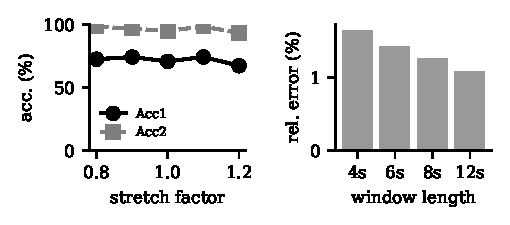
\includegraphics[width=\columnwidth]{../figures/fig_tempo_change.pdf}
\caption{Left: accuracy of the estimator with octave decision on time-stretched clips (\NChange{} clips). Right: median relative error of the local estimator for different window lengths.}
\label{fig:tchange}
\end{figure}

\begin{figure}[t]
\centering
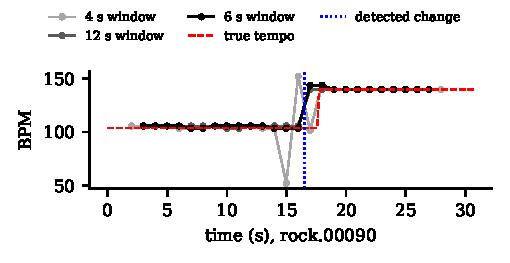
\includegraphics[width=\columnwidth]{../figures/fig_splice.pdf}
\caption{Local tempo of a clip spliced from parts stretched by 0.85 and 1.15, for three window lengths, with the true tempo and the detected change point.}
\label{fig:splice}
\end{figure}

\textbf{Objective 2: tempo estimation under tempo changes.}
\emph{PI1 (basic, done).} \NChange{} test clips were stretched by 0.8, 0.9, 1.0, 1.1 and 1.2. The factor 1.0 also goes through ffmpeg and checks that the processing itself does not change the result.
\emph{PI2 (basic, done).} All estimators were run on the stretched clips. Acc1 of the octave decision stays between \AccOneStretchMin{}\% and \AccOneStretchMax{}\% across factors (Figure~\ref{fig:tchange}), so a global change of tempo does not cause new octave errors, as long as the prior centre stays inside the octave of the music.
\emph{PI3 (expected, done).} The local estimator gives a median relative error of \RelErrTwelve{}\% with 12\,s windows and \RelErrFour{}\% with 4\,s windows on the stretched clips. Longer windows average more beats but react later to a change.
\emph{PI4 (expected, done).} On clips that jump from 0.85 to 1.15 times the original tempo at 15\,s, the 6\,s estimator has a median absolute error of \SpliceMAE{}\,BPM over the clip, and this error comes mostly from frames that jump an octave (Figure~\ref{fig:splice}). It settles within 4\% of the new tempo in \SettleFrac{}\% of the clips, with a median delay of \SettleMed{}\,s after the change. The delay is short because the window is centred on its time stamp and the new part quickly dominates it.
\emph{PI5 (advanced, done).} On \NChange{} clips spliced at a random time in both directions, the octave-folded detector finds the change with a median error of \DetFoldMed{}\,s and within 2\,s in \DetFoldTwo{}\% of the cases. Without folding, the octave jumps of the local estimate are taken as changes, and the error rises to \DetRawMed{}\,s (\DetRawTwo{}\% within 2\,s).

\textbf{What I learned and what did not work.} Octave errors are the main problem of tempo estimation, and a prior over typical tempi fixes more of them than a more complex pulse model. Our pulse trains need the normalisation and the extra features of the original paper \cite{percival}. For local tempo, octave jumps between windows are a larger error than the window length, and they also confuse change detection unless the curve is folded into one octave. The spliced clips are a controlled test only; real tempo changes are gradual, which our detector does not model yet.

\section{Team Status}
\label{sec:team}

\textbf{Nalluraj Babu} built the dynamic programming beat tracker of Ellis \cite{ellis} and tests it on degraded audio. The tracker reaches F = \DPF{} with the estimated tempo and \DPOracleF{} with the oracle tempo, against \LibF{} for librosa and \MadF{} for madmom (Table~\ref{tab:beats}). Given the same onset envelope and tempo, his tracker agrees with librosa's implementation at a median F of \AgreeRawMed{}, and \AgreeMed{} after adding librosa's envelope smoothing. Under degradation, the tracker is robust to MP3 and to moderate noise but loses accuracy with a 1\,kHz low pass filter (\DegLPOne{}) and with pink noise at $-10$\,dB (\DegNoiseMinusTen{}). The 1D State Space comparison and the advanced goals remain.

\textbf{Usha Sundaresan Manivannan} built a frame-wise neural network (an MLP on stacked log-mel features) and a downbeat finder that picks the bar position with the strongest bass and kick onsets. The MLP reaches F = \NNF{} with peak picking and \NNDBNF{} with madmom's DBN decoder on its own activation, which shows that the missing temporal model, not the frame classifier, causes most of its errors. For downbeats, the low-frequency finder reaches \DBOracle{} on annotated beats against \DBMadBar{} for madmom's bar tracker on the same beats and \DBMadJoint{} for madmom's joint model from audio. The TCN in PyTorch and the advanced goals remain.

\begin{table}[t]
\centering\small\setlength{\tabcolsep}{4pt}
\begin{tabular}{@{}lccc@{}}
\toprule
Beat tracker & F & CMLt & AMLt \\
\midrule
\csname @@input\endcsname ../figures/tab_beats.tex
\bottomrule
\end{tabular}
\caption{Beat tracking on the GTZAN test split (\NBeat{} clips).}
\label{tab:beats}
\end{table}

\PITable
\TimelineTable

\section{Revised Plan and Goals}

Our original plan assumed librosa, madmom and PyTorch from the start. Our first setup only had NumPy, SciPy and scikit-learn, so we built everything ourselves and moved the library comparisons later; these are now done for all three methods. Table~\ref{tab:pi} gives the status of every PI and Table~\ref{tab:time} the revised timeline.

\textbf{My goals for the final report.}
\emph{Basic:} add GiantSteps Tempo to PI2 and report all tempo results on both datasets.
\emph{Expected:} fix the pulse train stage with the normalisation of \cite{percival} and check whether it helps on top of the octave decision; run librosa and madmom on the stretched and spliced clips.
\emph{Advanced:} test the change detector on gradual tempo changes (a linear ramp of the stretch factor) and on GTZAN clips with real tempo drift, and compare with the predominant local pulse of \cite{plp}.

\textbf{Team goals.} Basic: every method and study complete on GTZAN. Expected: the TCN, the 1D State Space tracker in all comparisons, and GiantSteps. Advanced: tempo following and automatic tightness for the DP tracker, and a TCN with a downbeat output.

\section{Conclusion}

The tempo estimator works, and its main weakness, the octave error, is largely fixed by a simple prior. The tempo change study shows that a global change of speed is not a problem, but sudden changes produce octave jumps in short windows, which folding the tempo curve handles well enough to locate the change. The next steps are GiantSteps, a working pulse train stage and gradual tempo changes.

\begin{thebibliography}{99}\small\setlength{\itemsep}{0pt}
\bibitem{tutorial} M. E. P. Davies, S. B\"ock, and M. Fuentes, ``Tempo, beat and downbeat estimation,'' Tutorial at ISMIR, 2021. [Online]. Available: https://tempobeatdownbeat.github.io/tutorial
\bibitem{bello} J. P. Bello, L. Daudet, S. Abdallah, C. Duxbury, M. Davies, and M. Sandler, ``A tutorial on onset detection in music signals,'' \emph{IEEE Trans. Speech Audio Process.}, vol. 13, no. 5, pp. 1035--1047, 2005.
\bibitem{gouyon} F. Gouyon, A. Klapuri, S. Dixon, M. Alonso, G. Tzanetakis, C. Uhle, and P. Cano, ``An experimental comparison of audio tempo induction algorithms,'' \emph{IEEE Trans. Audio, Speech, Lang. Process.}, vol. 14, no. 5, pp. 1832--1844, 2006.
\bibitem{percival} G. Percival and G. Tzanetakis, ``Streamlined tempo estimation based on autocorrelation and cross-correlation with pulses,'' \emph{IEEE/ACM Trans. Audio, Speech, Lang. Process.}, vol. 22, no. 12, pp. 1765--1776, 2014.
\bibitem{ellis} D. P. W. Ellis, ``Beat tracking by dynamic programming,'' \emph{J. New Music Res.}, vol. 36, no. 1, pp. 51--60, 2007.
\bibitem{librosa} B. McFee, C. Raffel, D. Liang, D. P. W. Ellis, M. McVicar, E. Battenberg, and O. Nieto, ``librosa: Audio and music signal analysis in Python,'' in \emph{Proc. Python in Science Conf. (SciPy)}, pp. 18--25, 2015.
\bibitem{plp} P. Grosche and M. M\"uller, ``Extracting predominant local pulse information from music recordings,'' \emph{IEEE Trans. Audio, Speech, Lang. Process.}, vol. 19, no. 6, pp. 1688--1701, 2011.
\bibitem{downbeat} S. B\"ock, F. Krebs, and G. Widmer, ``Joint beat and downbeat tracking with recurrent neural networks,'' in \emph{Proc. ISMIR}, 2016.
\bibitem{madmom} S. B\"ock, F. Korzeniowski, J. Schl\"uter, F. Krebs, and G. Widmer, ``madmom: A new Python audio and music signal processing library,'' in \emph{Proc. ACM Multimedia}, pp. 1174--1178, 2016.
\bibitem{krebsbar} F. Krebs, S. B\"ock, M. Dorfer, and G. Widmer, ``Downbeat tracking using beat-synchronous features and recurrent neural networks,'' in \emph{Proc. ISMIR}, 2016.
\bibitem{tcn} M. E. P. Davies and S. B\"ock, ``Temporal convolutional networks for musical audio beat tracking,'' in \emph{Proc. EUSIPCO}, 2019.
\bibitem{heydari} M. Heydari, M. McCallum, A. Ehmann, and Z. Duan, ``A novel 1D state space for efficient music rhythmic analysis,'' in \emph{Proc. ICASSP}, 2022.
\bibitem{degradation} M. Mauch and S. Ewert, ``The Audio Degradation Toolbox and its application to robustness evaluation,'' in \emph{Proc. ISMIR}, pp. 83--88, 2013.
\bibitem{daviseval} M. E. P. Davies, N. Degara, and M. D. Plumbley, ``Evaluation methods for musical audio beat tracking algorithms,'' Queen Mary Univ. of London, Tech. Rep. C4DM-TR-09-06, 2009.
\bibitem{mireval} C. Raffel, B. McFee, E. J. Humphrey, J. Salamon, O. Nieto, D. Liang, and D. P. W. Ellis, ``mir\_eval: A transparent implementation of common MIR metrics,'' in \emph{Proc. ISMIR}, 2014.
\bibitem{gtzan} G. Tzanetakis and P. Cook, ``Musical genre classification of audio signals,'' \emph{IEEE Trans. Speech Audio Process.}, vol. 10, no. 5, pp. 293--302, 2002.
\bibitem{sturm} B. L. Sturm, ``The GTZAN dataset: Its contents, its faults, their effects on evaluation, and its future use,'' arXiv:1306.1461, 2013.
\bibitem{kereliuk} C. Kereliuk, B. L. Sturm, and J. Larsen, ``Deep learning and music adversaries,'' \emph{IEEE Trans. Multimedia}, vol. 17, pp. 2059--2072, 2015.
\bibitem{marchand} U. Marchand, Q. Fresnel, and G. Peeters, ``GTZAN-Rhythm: Extending the GTZAN test-set with beat, downbeat and swing annotations,'' in \emph{Late-Breaking Demo, ISMIR}, 2015.
\bibitem{giantsteps} P. Knees, \'A. Faraldo, P. Herrera, R. Vogl, S. B\"ock, F. H\"orschl\"ager, and M. Le Goff, ``Two data sets for tempo estimation and key detection in electronic dance music annotated from user corrections,'' in \emph{Proc. ISMIR}, 2015.
\end{thebibliography}

\end{document}
